The first subsection will explain the system's architecture in detail based on a \ac{UML} diagram. With this diagram, it is possible to show the component-based architecture and how the mentioned tools are combined for the different visualisations and concepts. The second subsection will show the transition manager in detail, which features the transition table mentioned in chapter \ref{s:theoretical-contrib} on page \pageref{s:theoretical-contrib}.
As already mentioned in chapter \ref{s:collaboration-statement} on page \pageref{s:collaboration-statement}, \citeauthor{Wanko2016} is researching on a related topic of this thesis. The practical part of his his thesis and the one of this thesis are implemented in the same system. Therefore, the actual application has a lot more features and options than described in this section.

\subsubsection{Application Architecture}
Figure \ref{fig:uml-practical-approach} on page \pageref{fig:uml-practical-approach} gives an overview of the architecture in the form of a class diagram. However, the diagram shown and discussed in the master-thesis of \citeauthor{Wanko2016} looks quite different, although it is based on the same system. This is due to the relatively big system architecture and the different scopes of both theses \iacite{Wanko2016}. Showing and discussing all available classes, features and options for the application would go beyong the scope. The following list will briefly discuss the most important classes and their purposes:

\begin{figure}[!htb]
\centering
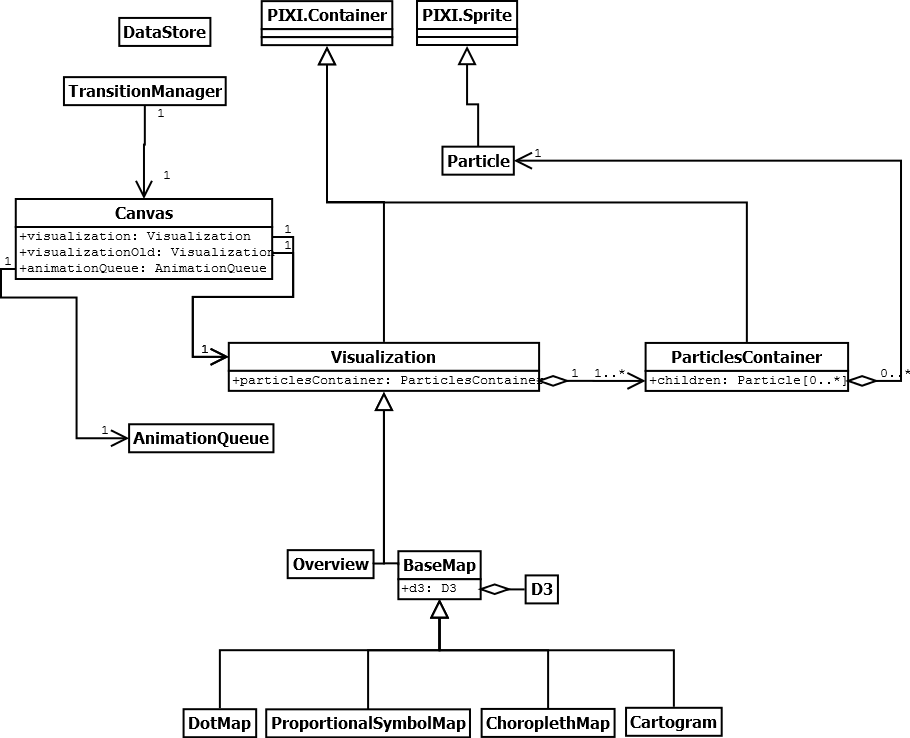
\includegraphics[width=0.8\textwidth,keepaspectratio]{images/results/dia.png}
% 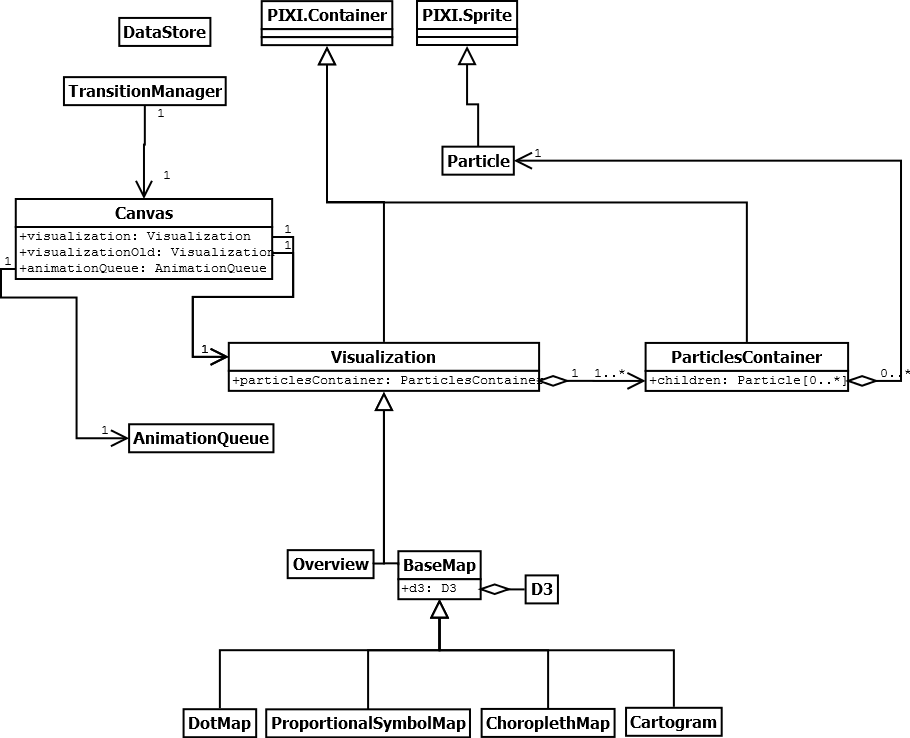
\includegraphics[height=10cm]{images/results/dia.png}
\caption[
    Overview of the application architecture in the form of a class diagram.
]{Overview of the application architecture in the form of a class diagram.}
\label{fig:uml-practical-approach}
\end{figure}


\begin{description}
\item[DataStore] \hfill \\
An object of the DataStore-class is used to load the SuperStore-Sale dataset. In addition to initally loading it, it also parses and analyses the dataset. Each attribute of the dataset got classified to handle the attributes correctly later on. For the sake of convenience, three different classification types were used: numeric, date, nominal and unknown.

\item[PIXI.Container] \hfill \\
\ac{Pixi} features functionalities like container classes. \textit{PIXI.Container} is such a class and can be used to put objects in it, and scale or move those objects according to the base-canvas.

\item[AnimationQueue] \hfill \\
If an animation is assigned to particles, it is stored in the \textit{AnimationQueue}. This allows to create multiple canvas-based animations and process them sequential.

\item[Canvas] \hfill \\
This class is one of the main classes inside the application. It is needed to not compare it with an HTML-Canvas object. However, this class is responsible for creating the base-canvas of the web-application. Furthermore, it is used to change and update the visual appearance if any interaction happens. A key part of the canvas class is the render function shown in listing \ref{lst:canvas-render} on page \pageref{lst:canvas-render}. It starts off with calling the same function again as soon as possible. The caller-function \textit{requestAnimationFrame} ensures, that the next frame will only be shown if enough resources of the browser are available. Afterwards, all particles and visualisations are animated if something changed. The last line of the listing shows the \ac{Pixi}-renderer. Listing \ref{lst:canvas-autodecet-renderer} on page \pageref{lst:canvas-autodecet-renderer} shows its creation. It features the main canvas-size, background transparency, antialiasing and a lot of other options.

\begin{lstlisting}[language=JavaScript, caption={Render function of the canvas class.}, label={lst:canvas-render}]
    render() {
      this.requestFrameID = requestAnimationFrame(this.render.bind(this));

      let areParticlesAnimating = this.particlesContainer.nextStep();
      let isNewVisualizationAnimating = this.visualization.nextStep();
      let isOldVisualizationAnimating =  ? this.visualizationOld.nextStep() : false;

      if (!areParticlesAnimating && !isOldVisualizationAnimating &&
        !isNewVisualizationAnimating && this.animationQueue.length > 0) {

        this.animationQueue.pop()();
        this.particlesContainer.startAnimation();
        this.visualization.startAnimation();
        if (this.visualizationOld){
            this.visualizationOld.startAnimation();
        }
      }
      this.renderer.render(this.stage);
    }
\end{lstlisting}

\begin{lstlisting}[language=JavaScript, caption={Pixi's autodetect-renderer.}, label={lst:canvas-autodecet-renderer}]
    this.renderer = PIXI.autoDetectRenderer(this.width, this.height, {
        transparent: true,
        clearBeforeRender: true,
        antialias: true
    });
    document.body.appendChild(this.renderer.view);
\end{lstlisting}

\item[Visualization] \hfill \\
This class is the starting point and the parent class for all other types of visualisations. It stores a reference to the \textit{ParticleContainer} and provides functionality to move, sclae or change visualisations.

\item[Overview] \hfill \\
Creating an instance of \textit{Overview} will show all data items as unit-based grid.

\item[D3] \hfill \\
This class is mainly used to wrap all functionality of the \ac{D3} library. It features functions like initializing the base-map as a \ac{SVG} and loading the needed TopoJSON data accordingly. Listing \ref{lst:d3-topojson} on page \pageref{lst:d3-topojson} features a key part of this class. It shows how TopoJSON is used on the client. The filter function passed to the first \textit{TopoJSON.mesh}-function specifies that only internal state borders should be drawn. Thus, coastlines will not be drawn to retain detail around small islands and inlets. The filter function passed to the second \textit{TopoJSON.mesh}-function extends the first one by only drawing each county boundary once. Thus, if two counties share the same border, it is only drawn once.

\begin{lstlisting}[language=JavaScript, caption={TopoJSON usage on the client with the adaption of merging all geographic information.}, label={lst:d3-topojson}]
        this.data.topojson.states = topojson.mesh(
            this.data.us,
            this.data.us.objects.states,
            (a, b) => {
                return a !== b;
            }
        );

        this.data.topojson.counties = topojson.mesh(
            this.data.us,
            this.data.us.objects.counties,
            (a, b) => {
                return (
                    a !== b &&
                    !(this.getCountyIdentifier(a) / 1000 ^ this.getCountyIdentifier(b) / 1000)
                );
            }
        );
\end{lstlisting}

Another important aspect of the \ac{D3} class is the \textit{calculateCentroids}-function shown in listing \ref{lst:d3-calculate-centroids} on page \pageref{lst:d3-calculate-centroids}. It calculates a look-up dictionary for the given level of detail for each data item. Thus, providing a huge performance boost when finding out the centroid of a unit later on.

\begin{lstlisting}[language=JavaScript, caption={Calculate a look-up dictionary for all data items depending on the level of detail.}, label={lst:d3-calculate-centroids}]
    calculateCentroids(levelOfDetail){
        const boundaries = this._topojson.feature(
            this.data.us,
            this.data.us.objects[levelOfDetail]
        ).features;

        this.centroids[levelOfDetail] = {};
        for(let boundary of boundaries){
            this.centroids[levelOfDetail][boundary.id] = this.path.centroid(boundary);
        }
    }
\end{lstlisting}

\item[BaseMap] \hfill \\
% , that each visualisation shares the same object of \ac{D3}. Thus, e.g. changing the level of detail of the base map will affect all upcoming visualisations because they all share the same object.

\item[DotMap] \hfill \\
\item[ProportionalSymbolMap] \hfill \\
\item[ChoroplethMap] \hfill \\
\item[Cartogram] \hfill \\
\item[ParticlesContainer] \hfill \\
\item[Particle] \hfill \\
\end{description}

% in order to create aggregated maps, it can be done through loading a file containing the information or dynamically calculate it; cross-reference needed i.o. to explain merging files with topojson

\subsubsection{Interaction}
% transition
% level of detail
% changing visual appearance